%! Author = danielmendes
%! Date = 29.11.24

\chapter{Indexierung}\label{ch:indexing}

Das folgende Kapitel befasst sich mit der Indexierung und den damit verbundenen Performance-Optimierungen, die näher erläutert werden.
Zunächst betrachten wir einige Grundlagen der Indexierung.
Anschließend lernen wir die verschiedenen Arten von Indizes näher kennen und führen unterschiedliche Benchmarks mit Ihnen durch.
Im letzten Schritt analysieren wir die Ergebnisse und stellen fest, welche Verwendung der Indizes am besten funktioniert.

\section{Grundlagen}\label{sec:indexing-grundlagen}

Indizes sind Datenstrukturen, die von Speicher-Engines (engl.\ storage engines) verwendet werden, um unter anderem Zeilen schneller zu finden (\cite[pp. 147--189]{schwartz2012high}).
Die Storage-Engine ist eine Kernkomponente eines Datenbankmanagementsystems, die für die Speicherung und Verwaltung der Daten verantwortlich ist.
Verschiedene Storage-Engines unterscheiden sich hinsichtlich ihrer Indexfunktionalität sowie der Unterstützung von Transaktionen und Sperrmechanismen.
Im weiteren Verlauf werden wir verschiedene Indextypen kennenlernen, die nicht von allen Engines unterstützt werden.

Die Indizes haben einen großen Einfluss auf die Datenbank-Performance und werden mit zunehmender Größe der Datenbank immer wichtiger, da das Scannen aller Tupel zunehmend aufwendiger wird.
Weniger ausgelastete Datenbanken können ohne ordnungsgemäße Indizes gut funktionieren, aber die Leistung kann rapide sinken, wenn die Datenmenge wächst.
Wenn ein solches Problem auftritt, ist die Index-Optimierung oft der effektivste Weg, um die Abfrageleistung schnell zu verbessern.
Um wirklich optimale Indizes zu erstellen, ist es häufig notwendig, Abfragen umzuschreiben.
Besonders nützlich sind Indizes bei Abfragen, die Joins zwischen mehreren Tabellen enthalten, da sie ermöglichen, die Anzahl der zu prüfenden Tupel erheblich zu reduzieren, wenn eine einschränkende Bedingung vorliegt.
Wie genau Indizes erstellt werden müssen, wird im Laufe dieses Kapitels geklärt.


Um die Funktionsweise eines Indexes anschaulicher zu erklären, betrachten wir als Beispiel ein wissenschaftliches Fachbuch.
Am Ende dieser Bücher gibt es meist ein Stichwortverzeichnis oder Register.
Dieses Register besteht aus einer alphabetisch geordneten Liste von Begriffen, Themen und Stichworten.
Möchte man einen Begriff nachschlagen, sucht man ihn im Stichwortverzeichnis und erhält die Seitenzahlen, auf denen er vorkommt.
In DBMS verwendet die Storage-Engine Indizes auf eine ähnliche Weise.
Sie durchsucht die Datenstruktur des Indexes nach einem Wert.
Und wenn ein Treffer gefunden wird, kann die Engine die Zeilen ermitteln, die den Treffer enthalten.
Betrachten wir dazu folgendes Beispiel:

\begin{lstlisting}[language=SQL]
SELECT NAME FROM KUNDEN WHERE KUNDEN_ID = 7;
\end{lstlisting}

Wenn wir annehmen, dass es einen Index auf der Spalte \texttt{KUNDEN\_ID} gibt, dann nutzt MySQL diesen, um Zeilen zu finden, deren \texttt{KUNDEN\_ID} gleich 7 ist.
Mit anderen Worten wird eine Suche innerhalb der Indexwerte durchgeführt und alle entsprechenden Zeilen werden zurückgegeben.

Ein Index kann Werte aus einer oder mehreren Spalten einer Tabelle enthalten.
Bei mehreren Spalten ist die Reihenfolge der Spalten im Index entscheidend, da MySQL nur effizient auf ein linkes Präfix des Indexes zugreifen kann.
Gibt man nur das zweite Attribut an, ohne das erste zu referenzieren, kann der Index nicht direkt verwendet werden.
Außerdem darf man nicht verwechseln, dass ein Index über zwei Spalten nicht gleichbedeutend ist mit zwei separaten einspaltigen Indizes.
Es gibt verschiedene Typen von Indizes, die jeweils für unterschiedliche Zwecke optimiert sind und in den nächsten Abschnitten behandelt werden.

Um zu verstehen, wie man Indizes für eine Datenbank auswählt, ist es wichtig zu wissen, welcher Teil der Abfrage am meisten Zeit in Anspruch nimmt (\cite[pp. 350--353]{garcia2008database}).
Das Datenbanksystem ist so aufgebaut, dass die Tupel einer Relation üblicherweise auf viele Seiten einer Festplatte verteilt sind, die jeweils mehrere Tausend Bytes umfassen und viele Tupel speichern.
Um die Werte eines Tupels zu prüfen, muss die gesamte Seite, auch Block genannt, in den Hauptspeicher geladen werden.
Dabei kostet es kaum mehr Zeit, alle Tupel einer Seite anstatt nur ein einzelnes zu prüfen.

In der Regel stellt der Schlüssel den sinnvollsten Index für eine Tabelle dar, weshalb MySQL standardmäßig den B-Tree-Index für Primary Keys verwendet (\cite{mysql_primary_key}).
Die Entscheidung, ob für ein bestimmtes Attribut ein Index definiert werden soll, hängt von drei Faktoren ab:
Erstens ist ein Index besonders nützlich, wenn Abfragen häufig auf ein bestimmtes Attribut zugreifen.
Zweitens kann ein Index sinnvoll sein, wenn es nur wenige Tupel für einen bestimmten Wert des Attributs gibt, da dies den Festplattenzugriff bei einer Abfrage reduziert.
Sobald nicht alle Blöcke geladen werden müssen, kann der Index Zeit sparen.
Der letzte Fall betrifft Situation, in denen Tupel nach einem Attribut geclustert sind.
Durch einen Index können müssen hier weniger Datenblöcke geladenen werden, da die Werte des Attributs aufeinanderfolgender gespeichert sind.
Mit diesen Faktoren können wir begründen, warum die Schlüssel einer Tabelle gut geeignet sind.
Zum einen kommen sie oft in Abfragen vor (erster Punkt) und zum anderen enthalten sie keine doppelten Werte, da jedes Tupel einen eindeutigen Wert hat (zweiter Punkt).

Das Auswählen von Indizes erfordert von den Entwicklern eine Tradeoff abzuwägen.
Es gibt dabei zwei Faktoren, die die Entscheidung beeinflussen.
Zum einen kann ein Index auf einem Attribut Abfragen mit diesem Attribut erheblich beschleunigen.
Zum anderen erschwert jeder Index Einfügungen, Löschungen und Aktualisierungen, da diese mehr Zeit und Aufwand erfordern.
Aber selbst wenn Modifikationen die häufigste Form von Datenbankaktionen sind, kann ein Index auf ein häufig verwendetes Attribut die Leistung verbessern.
Dies liegt daran, dass einige Modifikationsbefehle zuvor die Datenbank abfragen.
Im Kapitel \nameref{ch:partitions} wird uns dieses Thema wieder begegnen.

Um Zeitersparnis durch die Nutzung von Tupeln ohne vollständige Durchsuchung der Relation zu erreichen, müssen Indizes auf der Festplatte gespeichert werden.
Dies führt jedoch zu zusätzlichen Festplattenzugriffen.
Allgemein lässt sich sagen, dass Modifikationen in etwa doppelt so kostenintensiv sind wie der Zugriff auf den Index oder die Daten während einer Abfrage.
Damit wir berechnen können, ob sich ein Index für eine Spalte lohnt, müssen wir wissen, in welcher Wahrscheinlichkeit Abfragen und Modifikationen durchgeführt werden.

Um die Vorgehensweise anhand einer beispielhaften Berechnung durchzuführen, benutzen wir die folgende Tabelle (abgeändertes Beispiel aus~\cite[pp. 355--357]{garcia2008database}):
\vspace{-4pt}
\begin{lstlisting}
Fakten(Id, Bestelldatum, Artikel_Id, Kunden_Id, ...)
\end{lstlisting}
\vspace{-8pt}

Der Schlüssel der Faktentabelle ist die Spalte \texttt{Id} und für die Attribute \texttt{Artikel\_Id} und \texttt{Kunden\_Id} erstellen wir jeweils einen Index.
Damit haben wir inklusive des Primärschlüssels 3 unterschiedliche Indexe.
Als Nächstes brauchen wir Befehle, bei denen die Indexe benutzt werden (siehe~\ref{lst:indexing:fakten-select-insert-queries}).
In der ersten Zeile wird nur der Kundenindex verwendet, in der zweiten nur der Artikelindex und in der Letzten fügen wie eine Zeile ein.

\vspace{-12pt}
\begin{lstlisting}[language=SQL,caption=Select-Queries für die Faktentabelle,label={lst:indexing:fakten-select-insert-queries}]
SELECT Bestelldatum, Artikel_Id FROM Fakten WHERE Kunden_Id = k;
SELECT Bestelldatum, Kunden_Id FROM Fakten WHERE Artikel_Id = a;
INSERT INTO Fakten VALUES(i, b, a, k);
\end{lstlisting}
\vspace{-8pt}

Damit wir berechnen können, ob es sinnvoll ist, die Indizes zu erstellen, müssen wir bestimmte Voraussetzungen festlegen.
Zuallererst gehen wir davon aus, dass die Faktentabelle 10 Datenblöcke belegt und im Durchschnitt kauft jeder Kunde 3 Artikel und ein Artikel wird von 3 Kunden gekauft.
Die Tupel für einen bestimmten Kunden oder Artikel sind gleichmäßig über die 10 Seiten verteilt.
Trotzdem sind mit einem Index nur 3 Festplattenzugriffe erforderlich, um die durchschnittlich 3 Tupel für einen Kunden oder Artikel zu finden.
Dazu ist ein Festplattenzugriff erforderlich, um die Seite des Indexes zu lesen und ein weiterer, um die modifizierte Seite zurückzuschreiben, falls eine Indexseite geändert werden muss.
Haben wir keinen Index, sind 10 Festplattenzugriffe zum Lesen und zwei Festplattenzugriffe für Schreiben erforderlich.
Mit diesen Bedingungen kommen wir zu folgender Kostentabelle:

\vspace{-18pt}
\begin{table}[H]
    \centering
    \setlength{\arrayrulewidth}{0.4mm}
    \[
        \begin{array}{r|c c c c}
            \textbf{Aktion} & \textbf{Kein Index} & \textbf{Kunden Index} & \textbf{Artikel Index} & \textbf{Beide Indizes} \\ \hline
            Q_1 & 10 & 4 & 10 & 4 \\
            Q_2 & 10 & 10 & 4 & 4 \\
            I   & 2  & 4  & 4  & 6 \\ \hline
            \textbf{Durchschnitt} & 2 + 8p_1 + 8p_2 & 4 + 6p_2 & 4 + 6p_1 & 6-2p_1-2p_2 \\
        \end{array}
    \]
    \vspace{-5pt}
    \caption[Performance-Vergleich]{Kosten der unterschiedlichen Queries in Abhängigkeit der Indizes}
    \label{tab:performance-queries}
\end{table}
\vspace{-25pt}

Die letzte Zeile aus Tabelle~\ref{tab:performance-queries} gibt die durchschnittlichen Kosten einer Aktion an.
Unter der Annahme, dass der Anteil der Zeit, in der wir die erste Abfrage ausführen, p1 beträgt und der Anteil der Zeit für die zweite Query p2 ist.
Da die gesamte Zeit in einem System 100\% ausmacht, beträgt der Anteil der Zeit, in der wir I ausführen: 1 — p1 — p2.
Den Durchschnitt für den Kundenindex berechnen wir wie folgt:
\[
    4p_{1} + 10p_{2} + 4 \cdot (1 - p_{1} - p_{2}) = 4p_{1} + 10p_{2} + 4 - 4p_{1} - 4p_{2} = 4 + 6p_{2}
\]

Abhängig von den Werten für p1 und p2 kann jede der vier Optionen die geringsten Kosten für die drei Operationen verursachen.
Zum Beispiel, wenn p1 = p2 = 0,1, dann ist der Ausdruck 2 + 8pi + 8p2 am kleinsten, sodass wir keine Indizes bevorzugen würden.
Wenn jedoch p1 = 0,5 und p2 = 0,1 gelten, ergibt ein Index für die Kunden den besten Durchschnittswert.

Damit haben wir gezeigt, dass es sinnvoll ist, keinen Index zu verwenden, wenn überwiegend Einfügungen durchgeführt werden und nur sehr wenige Abfragen anfallen.
Intuitiv, wenn wir viele Abfragen durchführen und die Anzahl der Abfragen, die Artikel und Kunden angeben, ungefähr gleich häufig sind, dann sind beide Indizes erwünscht.
Wenn wir nur ein Typ von Query häufig verwenden, dann sollten wir nur den Index definieren, der uns bei dieser hilft.

Es gibt zahlreiche Tools, die entwickelt wurden, um die Verantwortung der Wahl der Indizes vom Datenbankdesigner zu übernehmen.
Dabei optimiert das System sich selbst oder dem Designer werden zumindest Empfehlungen für sinnvolle Entscheidungen gegeben.
Ein bewährter Ansatz zur Auswahl von Indizes ist das sogenannte Greedy-Verfahren (\cite{greedy_varfahren}), bei dem zunächst ohne ausgewählte Indizes der Nutzen jedes Kandidaten-Index bewertet wird.
Wenn es einen Index mit positivem Nutzen gibt, wird dieser ausgewählt und anschließend wird eine Neubewertung ausgeführt, wobei davon ausgegangen wird, dass der zuvor ausgewählte Index bereits verfügbar ist.
Dieser Prozess wird so lange wiederholt, bis es keinen Kandidaten-Index mit positivem Nutzen mehr gibt.

\newpage
\section{B-Baum-Index}\label{sec:indexing-b-baum-index}

Der erste zu betrachtende Indextyp ist der B-Baum-Index (engl.\ B-Tree Index), der auf einer speziellen Baum-Datenstruktur basiert.
Diese Struktur wird von den meisten MySQL-Storage-Engines unterstützt.
Die Implementierung und Nutzung des B-Baum-Indexes kann jedoch je nach verwendeter Storage-Engine variieren.

Das Grundprinzip eines B-Baums ist, dass alle Werte in einer bestimmten Reihenfolge gespeichert werden und jede Blattseite den gleichen Abstand zum Wurzelknoten hat.
Ein B-Baum-Index beschleunigt den Datenzugriff, da die Storage-Engine nicht die gesamte Tabelle durchsuchen muss, um die gewünschten Daten zu finden.
Stattdessen beginnt die Suche beim Wurzelknoten.

Die Slots im Wurzelknoten enthalten Zeiger auf Kindknoten und die Storage-Engine folgt diesen Zeigern.
Der richtige Zeiger wird durch Vergleich der Werte in den Knoten-Seiten (engl.\ node pages) ermittelt, die die oberen und unteren Grenzen der Werte in den Kindknoten definieren.
Letztlich stellt die Storage-Engine fest, ob der gewünschte Wert existiert oder ob sie erfolgreich eine Blatt (engl.\ leaf page) erreicht.

\vspace{-8pt}
\begin{figure}[H]
    \centering
    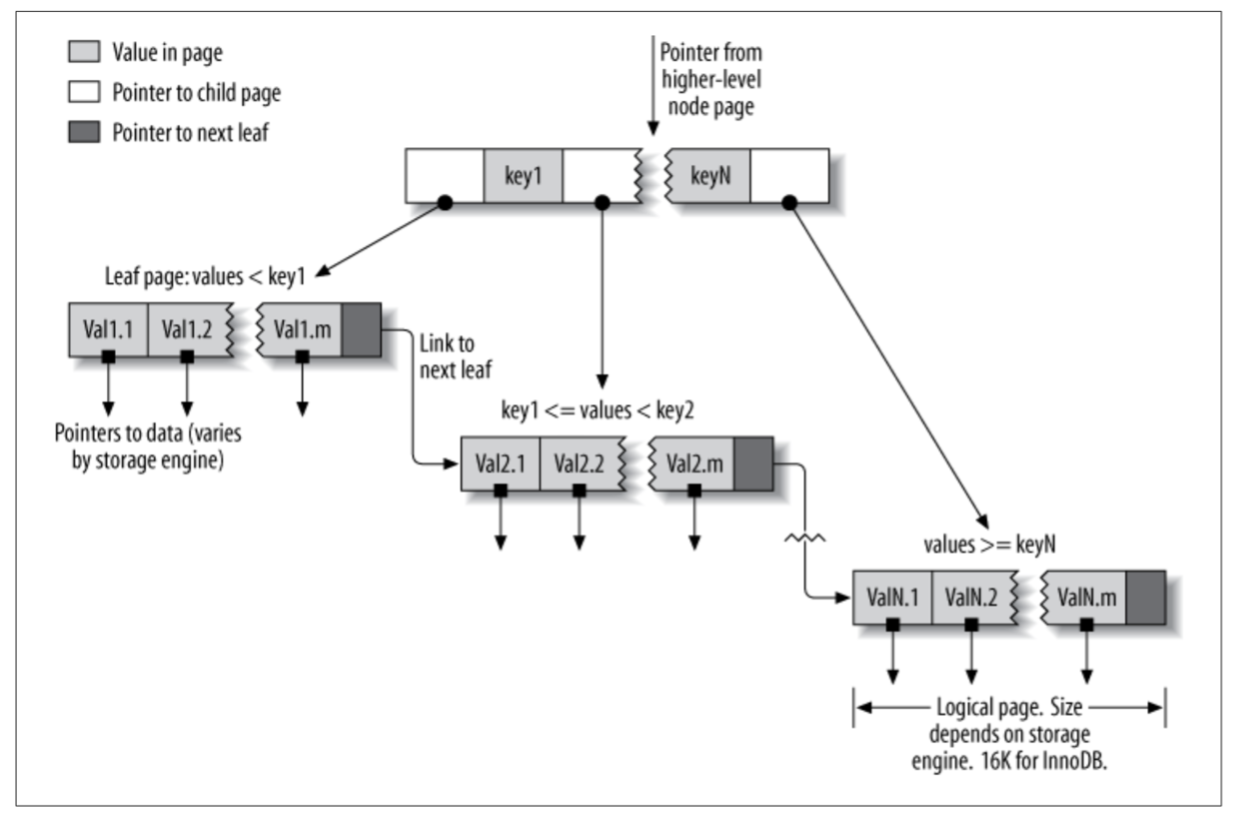
\includegraphics[width=0.65\textwidth]{PNGs/Textbook/B_Tree_Visualisation}
    \caption[Binärbaum-Visualisierung]{Binär-Baums-Darstellung (Abbildung 5--1 aus \cite[S. 149]{schwartz2012high})}
    \label{fig:b-tree-visualisation}
\end{figure}
\vspace{-20pt}

Die Blätter sind besonders, da sie Zeiger auf die indexierten Daten enthalten, anstatt auf andere Seiten zu verweisen.
Zwischen dem Wurzelknoten und den Blattseiten können viele Ebenen von Knoten-Seiten existieren.
Die Tiefe des Baumes hängt von der Größe der Tabelle ab.
Außerdem speichern B-Bäume die indexierten Spalten in einer festgelegten Reihenfolge, was sie besonders nützlich für die Suche nach Datenbereichen macht.
Beispielsweise kann ein Index auf einem Textfeld (z.B.\ vom Typ \texttt{VARCHAR}) effizient alle Namen finden, die mit „K“ beginnen, da die Werte in alphabetischer Reihenfolge gespeichert sind.

Der Index sortiert die Werte entsprechend der Reihenfolge der in der \texttt{CREATE INDEX}-Anweisung angegebenen Spalten, beispielsweise kann man wie folgt ein Index erstellen:

\vspace{-5pt}
\begin{lstlisting}[language=SQL,caption=B-Baum-Index bestehend aus mehreren Attributen,label={lst:indexing-create-combined}]
CREATE INDEX combined_index ON KUNDEN(NAME, VORNAME, GEBURTSTAG);
\end{lstlisting}
\vspace{-8pt}

Als Nächstes betrachten wir die möglichen Abfragen, bei denen B-Baum-Indizes besonders hilfreich sind, um ein besseres Verständnis für ihre optimale Nutzung zu erlangen.
Eine Übereinstimmung mit dem vollständigen Schlüsselwert liefert Werte für alle Spalten im Index.
Eine beispielhafte Abfrage zur Suche nach allen Einträgen mit dem Index aus~\ref{lst:indexing-create-combined} ist die Suche nach allen Kunden, die Max Mustermann heißen und am 01.01.2000 geboren wurden.
Auch Abfragen, die nur mit dem linken Präfix übereinstimmen, können von diesem Index profitieren.
So lässt sich etwa gezielt nach dem Nachnamen „Mustermann“ suchen.
Ebenso ist es möglich, nur ein Spaltenpräfix zu verwenden, etwa um alle Nachnamen zu finden, die mit „M“ beginnen.
Ein weiterer Vorteil ergibt sich bei Bereichsabfragen, denn der Index kann effizient genutzt werden, um Nachnamen zwischen „Mustermann“ und „Müller“ zu ermitteln.
Darüber hinaus unterstützt ein B-Baum-Index auch Kombinationen aus exakten und Bereichsabfragen, beispielsweise wenn nach dem Nachnamen „Mustermann“ gesucht wird, während der Vorname innerhalb eines Bereichs liegt, etwa ab „Ma“.
Ein weiterer Vorteil von B-Baum-Indizes ist, dass sie aufgrund der sortierten Baumstruktur nicht nur Abfragen, sondern auch \texttt{ORDER BY}-Bedingungen effizient unterstützen können.

Es gibt jedoch Einschränkungen von B-Baum-Indizes, die dazu führen, dass andere Indextypen für bestimmte Szenarien besser geeignet sind.
Eine Einschränkung ist, dass die Suche nicht am rechten Ende des Indexes beginnen kann.
Beispielsweise ist der Beispiels-Index nicht dazu geeignet, alle Personen zu finden, die vor dem Jahr 2000 geboren wurden, ohne dass der Nachname und Vorname ebenfalls spezifiziert werden.
Für optimale Leistung kann es auch erforderlich sein, dass Indizes mit den gleichen Spalten, jedoch in unterschiedlicher Reihenfolge erstellt werden.
Auf diese Weise könnten mehr Kombinationen abgedeckt und zusätzlich einige Abfragen optimiert werden.

Im nächsten Abschnitt führen wir die Benchmarks durch, um das Verständnis für die Funktionsweise des B-Baum-Indexes zu bestätigen.
Dafür erstellen wir zunächst wieder die Kundentabelle (\ref{lst:tools-create-table-kunde}) und definieren für den ersten Vergleich folgende Indizes:

\vspace{-5pt}
\begin{lstlisting}[language=SQL,caption=Definition mehrere Indizes,label={lst:indexing-create-multiple}]
CREATE INDEX idx_stadt ON KUNDEN(STADT);
CREATE INDEX idx_postleitzahl ON KUNDEN(POSTLEITZAHL);
CREATE INDEX idx_geburtstag ON KUNDEN(GEBURTSTAG);
\end{lstlisting}
\vspace{-5pt}

Um die Effizienz dieser Indizes einordnen zu können, vergleichen wir diese Konfiguration mit einer, bei der nur die Kundentabelle ohne Indizes erstellt wird.
In beiden Fälle werden eine bestimmte Anzahl an Datensätze eingefügt.
Um die Performance der Select-Abfragen zu messen, führen wir verschiedene Queries an die Datenbank aus, bei denen die Attribute \texttt{GEBURTSTAG}, \texttt{STADT} und \texttt{POSTLEITZAHL} berücksichtigt werden.
Dazu gehören \texttt{GROUP BY}- und \texttt{COUNT}-Abfragen, bei denen die Index-Attribute verwendet werden oder sie spielen in der \texttt{WHERE}-Bedingung eine Rolle.
Damit es übersichtlich bleibt, vergleichen wir einmal 10 Datensätze mit 40 und einmal 400 mit 4000 Zeilen.

\begin{figure}[H]
    \centering
    \begin{subfigure}[t]{0.48\textwidth}
        \centering
        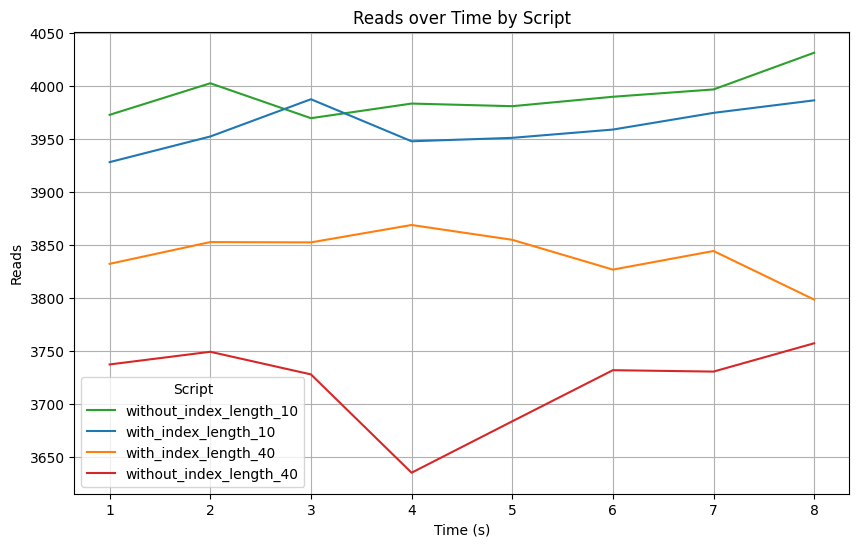
\includegraphics[width=\textwidth]{PNGs/Script/Index/B_Tree/low-count/Reads}
        \caption{Mit 10 und 40 Datensätze}
        \label{indexing-b-tree-low-reads}
    \end{subfigure}
    \hfill
    \begin{subfigure}[t]{0.48\textwidth}
        \centering
        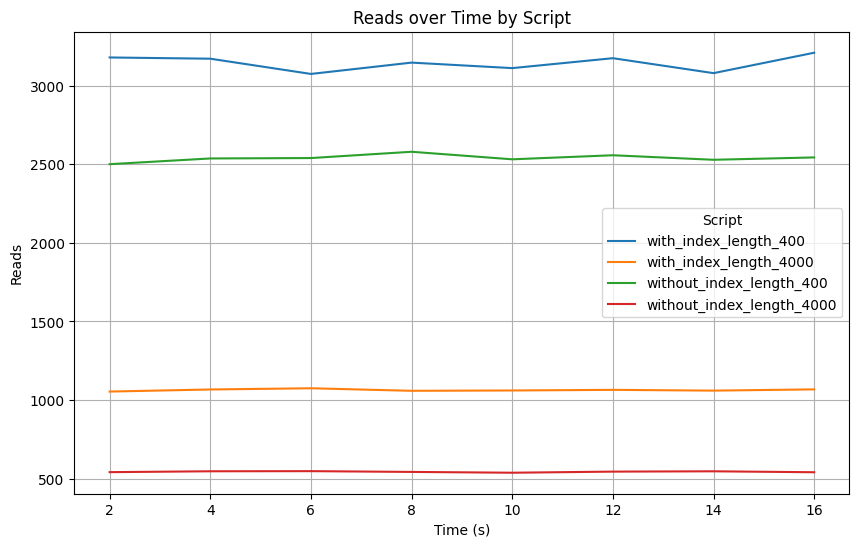
\includegraphics[width=\textwidth]{PNGs/Script/Index/B_Tree/high-count/Reads}
        \caption{Mit 400 und 4000 Zeilen}
        \label{indexing-b-tree-high-reads}
    \end{subfigure}
    \caption[B-Tree-Indexing: Mit Index vs Ohne]{Grafik zeigt Performance mit und ohne Index für Readsabfragen}
    \label{fig:indexing-vs-no}
\end{figure}
\vspace{-15pt}

In der Abbildung~\ref{indexing-b-tree-low-reads} können wir erkennen, dass bei 10 Datensätzen die Kundentabelle ohne Indizes schneller ist als diejenige mit.
Bei 40, 400 oder 4000 (siehe~\ref{indexing-b-tree-high-reads}) Zeilen sehen wir schon die Wirkung, die die Indizes haben können, denn dort ist jeweils die Version mit Indizes effizienter.
Der Unterschied bei 40 Datensätzen ist zwar etwas geringer, aber in den anderen Fällen sehen noch eindeutigere Unterschiede.
Interessant ist, dass es nicht linear oder quadratisch mit der Anzahl an Datensätzen in der Tabelle steigt, sondern bei 400 und 4000 Zeilen beträgt der Unterschied zur Tabelle ohne Index jeweils etwa 500--700 Abfragen.
Bei der Schreibgeschwindigkeit liegen beide auf einem sehr ähnlichen Niveau, wobei die Version ohne Index tendenziell einen leichten Vorteil hat.

Mit dem vorherigen Benchmark können wir die Vorteile eines Indexes schon deutlich erkennen.
Jetzt wollen wir aber auch die Funktionalität des B-Tree-Indexes in Bezug auf unterschiedliche Selects untersuchen.
Dazu erstellen wir erneut die Kundentabelle, aber dieses Mal definieren wir nur einen Index (siehe~\ref{lst:indexing-create-combined}).
Anschließend befüllen wir die Tabelle mit einer festgelegten Anzahl an Datensätzen und führen unterschiedliche Select-Befehle aus.
Im Codeblock~\ref{lst:indexing-b-tree-selects} sehen wir aus Platzgründen nur die Where-Bedingung und am Ende jeder Zeile steht der Name der Query, damit wir später in der Analyse wissen, welcher Query welche Performance bringt.

\newpage
\begin{lstlisting}[language=SQL,caption=Unterschiedliche Where-Bedingungen für B-Tree-Index,label={lst:indexing-b-tree-selects},basicstyle=\ttfamily\scriptsize]
WHERE NAME LIKE 'M%'; -- columm_prefix
WHERE NAME = 'Müller' AND VORNAME = 'Max' AND GEBURTSTAG < '1980-01-01'; -- combined_match_with_range
WHERE NAME = 'Müller' AND VORNAME LIKE 'M%' ORDER BY GEBURTSTAG; -- exact_with_prefix
WHERE NAME = 'Müller' AND VORNAME = 'Max' AND GEBURTSTAG = '1960-01-01'; -- full_match
WHERE NAME = 'Müller'; -- leftmost_prefix
WHERE GEBURTSTAG < '1980-01-01'; -- not_leftmost
WHERE NAME BETWEEN 'Müller' AND 'Schulz'; -- range_values
WHERE NAME = 'Müller' AND VORNAME LIKE 'M%' AND GEBURTSTAG < '1980-01-01'; -- range_with_like
WHERE NAME = 'Müller' AND GEBURTSTAG < '1980-01-01'; -- skip_columns
\end{lstlisting}
\vspace{-5pt}

Anhand der Grafik in Abbildung~\ref{fig:indexing-b-tree-query-reads} lässt sich erkennen, bei welchen Abfragen der Index am effizientesten ist.
Auf der linken Seite können wir die Ergebnisse für die Read-Befehle mit Index betrachten und auf der rechten Seite die Werte ohne Index.

\vspace{-5pt}
\begin{figure}[H]
    \centering
    \begin{subfigure}[t]{0.48\textwidth}
        \centering
        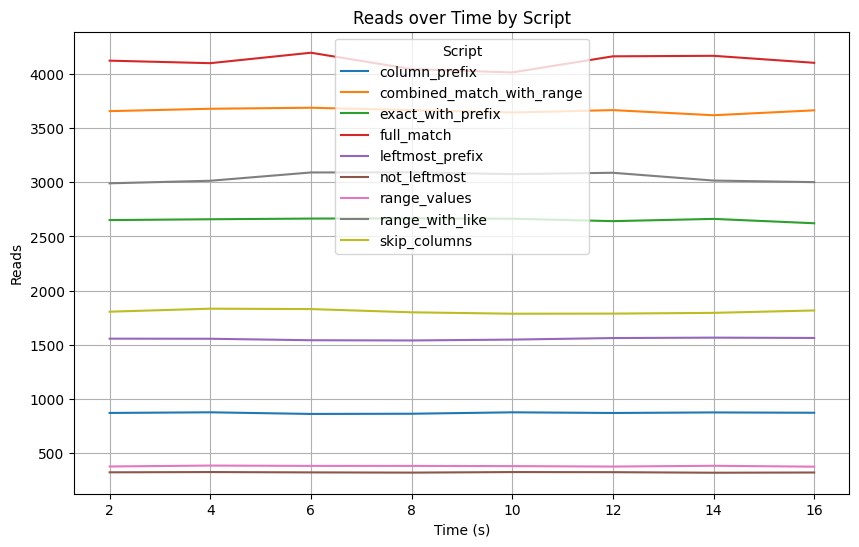
\includegraphics[width=\textwidth]{PNGs/Script/Index/B_Tree/b-tree-query-differences/Reads}
        \caption{Mit Index}
        \label{indexing-b-tree-query-reads-index}
    \end{subfigure}
    \hfill
    \begin{subfigure}[t]{0.48\textwidth}
        \centering
        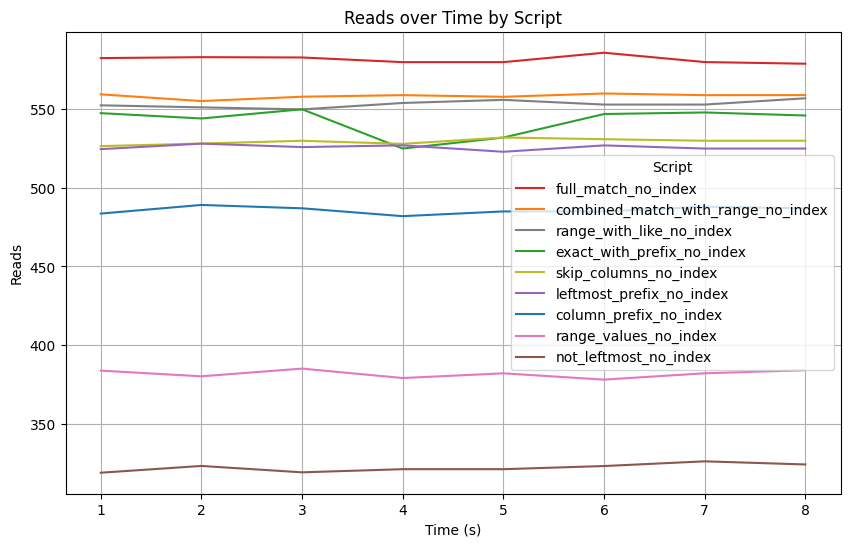
\includegraphics[width=\textwidth]{PNGs/Script/Index/B_Tree/b-tree-query-differences-no-index/Reads}
        \caption{Ohne Index}
        \label{indexing-b-tree-query-reads-no-index}
    \end{subfigure}
    \vspace{-5pt}
    \caption[B-Tree-Indexing: Unterschiedliche Selects mit Index und Ohne]{Visualisierung von unterschiedlichen Select-Queries mit und ohne Index}
    \label{fig:indexing-b-tree-query-reads}
\end{figure}
\vspace{-15pt}

Zunächst fällt auf, dass die Reihenfolge für die Werte mit und ohne Index komplett identisch ist.
Dies ist direkt erkennbar, da die Legenden beider Grafiken nach dem durchschnittlichen Wert über die gesamte Zeit sortiert sind.
Damit wir aber die richtigen Schlüsse aus der Grafik ziehen können, müssen wir herausfinden, wie viele Zeilen die unterschiedlichen Queries zurückgeben.
Dazu führen wir die Abfragen zusätzlich mit dem \texttt{COUNT(*)}-Operator durch und schreiben die Ergebnisse auch in die log-Datei.
Anschließend entnehmen wir die Werte und fügen sie in einer Tabelle zusammen.

\vspace{-5pt}
\begin{table}[H]
    \centering
    \scriptsize
    \begin{tabular}{|l|l|l|l|}
        \hline
        \textbf{Select-Query} & \textbf{Anzahl an Zeilen} & \textbf{Faktor} & \textbf{Index benutzt?} \\
        \hline
        full\_match & 0 & 6.42 & ja \\
        combined\_match\_with\_range & 13 & 5.78 & ja \\
        range\_with\_like & 31 & 5.22 & ja \\
        exact\_with\_prefix & 51 & 5.14 & ja \\
        skip\_columns & 147 & 3.47 & ja \\
        leftmost\_prefix & 263 & 2.73 & ja \\
        column\_prefix & 551 & 1.69 & ja \\
        range\_values & 1343 & 0.96 & nein \\
        not\_leftmost & 2371 & 0.98 & nein \\
        \hline
    \end{tabular}
    \vspace{3pt}
    \caption{Ergebnisse der COUNT(*)-Abfragen für B-Tree-Index}
    \label{tab:indexing_b_tree_count_results}
\end{table}
\vspace{-25pt}

Anhand der Spalte \texttt{Anzahl an Zeilen} können wir erkennen, dass die Queries, die am wenigsten Zeilen zurückgeben, auch diejenigen sind, bei denen es die höchste Performance gibt.
Deshalb ist auch die Reihenfolge mit und ohne Index gleich, weshalb man meinen könnte, dass der Index keinen Einfluss auf die Performance hat.
Dies betrifft aber nur die Reihenfolge, nicht jedoch die Werte der Abfragen, da wir hier deutliche Unterschiede sehen.
Anschaulich wird das mit der Betrachtung der Spalte \texttt{Faktor}.
Um den Wert zu berechnen, entnehmen wir die Werte aus der Gesamtstatistik und teilen die mit Index durch die ohne Index.
Damit können wir sehen, dass \texttt{full\_match} zwar bei beiden Versionen am schnellsten im Vergleich ist, aber mit Index etwa 6-mal schneller als ohne ist.
Es lässt sich auch erkennen, dass je weniger Zeilen zurückgegeben werden, desto größer ist der Faktor.
Bei den Queries \texttt{range\_values} und \texttt{not\_leftmost} liegt der Faktor sehr nah 1, was bedeutet, dass der Index keinen Einfluss auf die Performance hat.
Deshalb stellt sich auch die Frage, ob der Index überhaupt verwendet wird.
Um das zu überprüfen, verwenden wir den \texttt{EXPLAIN}-Operator, loggen wieder das Ergebnis und fügen es der Tabelle hinzu (siehe Spalte \texttt{Index benutzt?}).
Und tatsächlich sehen wir, dass die vermuteten Queries die einzigen sind, bei denen der Index nicht verwendet wird.

\section{Hash-Index}\label{sec:indexing-hash-index}
Ein weiterer Indextyp, den wir betrachten, ist der Hash-Index.
Dieser basiert auf einer Hash-Tabelle und ist daher nur für exakte Suchanfragen geeignet, die alle Spalten des Indexes verwenden.
In MySQL unterstützt nur die Memory-Storage-Engine explizite Hash-Indizes.
Einige Storage-Engines, wie zum Beispiel InnoDB, können erkennen, wenn bestimmte Index-Werte besonders häufig abgefragt werden.
Sie erstellen dann automatisch einen Hash-Index für diese Werte im Speicher, der zusätzlich zu den bestehenden B-Baum-Indizes genutzt wird.
Die Funktionsweise der Storage-Engine lässt sich wie folgt beschreiben.

Für jede Zeile wird mithilfe einer Hash-Funktion ein Hash-Wert der indexierten Spalte berechnet.
Der Hash-Wert (engl.\ hash code) ist eine kleine Zahl, die sich in der Regel von den Hash-Werten anderer Zeilen mit unterschiedlichen Schlüsselwerten unterscheidet.
Anschließend wird die Position im Index gesucht und man findet einen Zeiger auf die entsprechende Zeile.
In letzten Schritt überprüft man die Werte der Zeile, um sicherzustellen, dass es sich um die richtige Zeile handelt.

Wenn mehrere Werte denselben Hash-Wert besitzen, speichert der Index die Zeiger auf die Zeilen (engl.\ row pointers) in demselben Hash-Tabelleneintrag, typischerweise mithilfe einer verketteten Liste (z.B.\ einer \textit{Linked List}).
Hash-Kollisionen können die Leistung eines Hash-Index beeinträchtigen, da jeder Zeiger in der verketteten Liste durchlaufen und die entsprechenden Werte mit dem Suchwert verglichen werden müssen, um die richtigen Zeilen zu finden.
Das ist auch Index-Wartungsoperationen mit viel Aufwand verbunden.
Hingegen eindeutige Hash-Indizes stellen sicher, dass für jeden Hash-Wert nur ein einziger Eintrag existiert.
Bei Konflikten wird ein Mechanismus wie die Open Addressing-Strategie (z.B.\ Linear Probing oder Quadratic Probing) eingesetzt, um Konflikte zu lösen und den Speicherplatz effizient zu verwalten.
Hierbei wird versucht, Konflikte direkt innerhalb der Hash-Tabelle zu bewältigen, anstatt auf zusätzliche Datenstrukturen wie verkettete Listen zurückzugreifen.
Die eindeutigen Hash-Indizes werden nicht von der Memory-Engine in MySQL unterstützt.

Um die Verwendung des Hash-Indexes zu veranschaulichen, benutzen folgt folgendes Beispiel:

\vspace{-5pt}
\begin{lstlisting}[language=SQL]
SELECT * FROM KUNDEN WHERE NAME = 'Peter';
\end{lstlisting}
\vspace{-8pt}

Zunächst berechnet MySQL den Hash-Wert für \texttt{'Peter'} und verwendet diesen, um den entsprechenden Zeiger im Index zu finden.
Angenommen, die Hash-Funktion liefert für \texttt{'Peter'} den Wert \textbf{7654}.
MySQL sucht nun im Index an der Position 7654 und findet einen Zeiger auf Zeile 3.
Im letzten Schritt wird der Wert in Zeile 3 mit \texttt{'Peter'} verglichen.
Da die Indizes nur kompakte Hash-Werte speichern, sind Hash-Indizes äußerst platzsparend und Suchvorgänge erfolgen in hoher Geschwindigkeit.

Ähnlich wie der B-Baum-Index hat auch der Hash-Index einige Einschränkungen.
Zum einen enthält der Index nur Hash-Werte und Zeiger auf Zeilen (engl.\ row pointers), jedoch nicht die Werte selbst.
Deshalb kann MySQL den Index nicht verwenden, um das Einlesen der Zeilen zu vermeiden.
Allerdings erfolgt der Zugriff auf die in den Speicher geladenen Zeilen sehr schnell, wodurch die Leistung nicht wesentlich beeinträchtigt ist.
Zum anderen können Hash-Indizes nicht für Sortierungen verwendet werden, da die Werte nicht in einer geordneten Reihenfolge gespeichert sind.
Im Gegensatz dazu sind B-Baum-Indizes in der Lage.
Darüber hinaus ermöglichen Hash-Indizes keine partiellen Schlüsselübereinstimmungen (engl.\ partial key matching).
Da der Hash-Wert aus dem gesamten indexierten Wert berechnet wird, hilft ein Hash-Index beispielsweise nicht, wenn ein Index aus den Spalten (A, B) besteht und die \texttt{WHERE}-Klausel nur auf A verweist.
Ein weiterer Nachteil besteht darin, dass Hash-Indizes keine Bereichsabfragen unterstützen.
Sie eignen sich lediglich für Gleichheitsvergleiche, wie die Operatoren \texttt{=} (gleich), \texttt{<=>} (null-sicher gleich) und \texttt{IN()}.

Als Nächstes kommen wir zu den Benchmarks mit Hash-Indizes.
Dazu verwenden wir erneut die Kundentabelle und erstellen nur einen Index für die Spalte \texttt{NAME}.
Am Ende des \texttt{CREATE INDEX}-Befehl müssen wir \texttt{USING HASH} hinzufügen, damit anstelle des standartmäßigen B-Tree-Index der Hash-Index verwendet wird.
Danach befüllen wieder die Tabelle mit Testdaten.

Diesmal untersuchen wir beim ersten Benchmark den Einfluss von Hash-Kollisionen für die Performance.
Um den Grad der Kollisionen zu verändern haben wir eine Variable, die die obere Grenze für die zufällige Generierung einer Zahl, darstellt.
Anschließend fragen wir alle Zeilen mit dem Wert \texttt{Kunde\_1} für die Spalte \texttt{NAME} ab und führen die Tests mit den Kollisionswahrscheinlichkeiten von 25\%, 10\%, 5\% und 1\% durch.

\begin{figure}[H]
    \centering
    \begin{subfigure}[t]{0.48\textwidth}
        \centering
        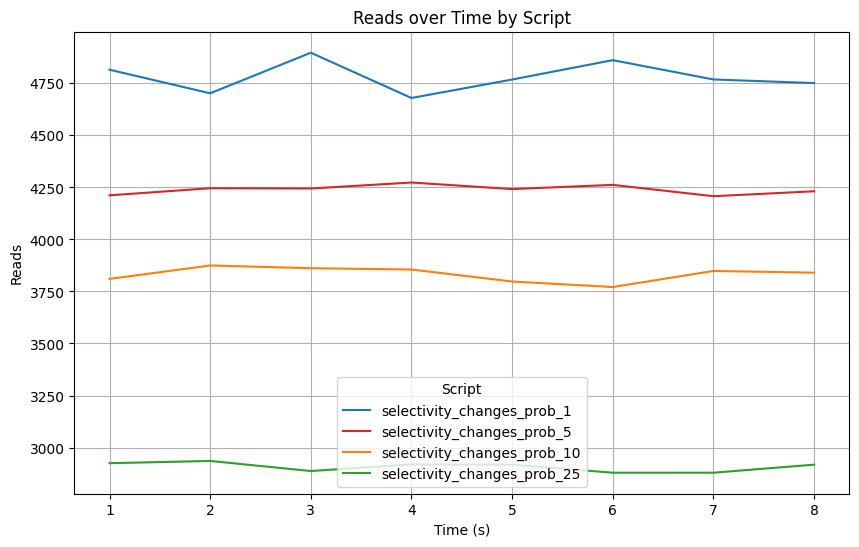
\includegraphics[width=\textwidth]{PNGs/Script/Index/Hash/selectivity-change/Reads}
    \end{subfigure}
    \hfill
    \begin{subfigure}[t]{0.48\textwidth}
        \centering
        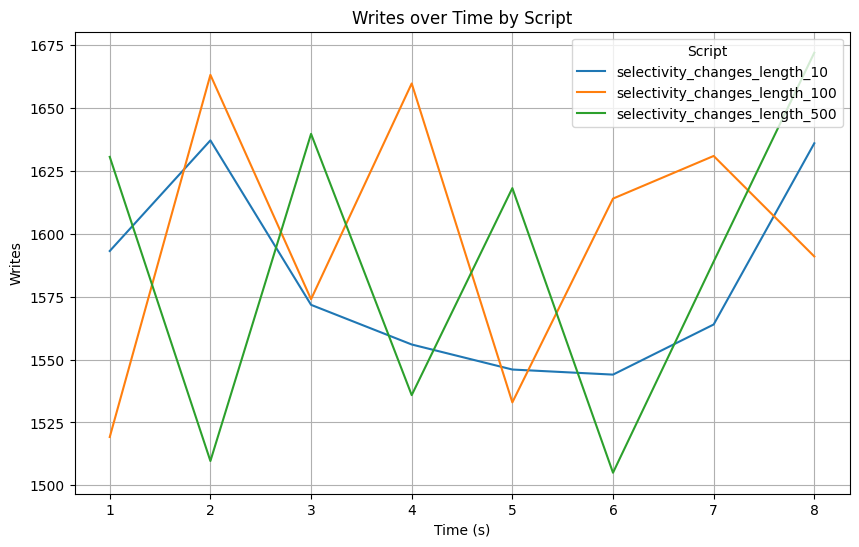
\includegraphics[width=\textwidth]{PNGs/Script/Index/Hash/selectivity-change/Writes}
    \end{subfigure}
    \vspace{-8pt}
    \caption[Hash-Indexing: Auswirkungen von Hashkollisionen]{Vergleich der Auswirkungen von Hashkollisionen}
    \label{fig:hash-collision-comparison}
\end{figure}
\vspace{-17pt}

An den Ergebnissen in Abbildung~\ref{fig:hash-collision-comparison} können wir sehen, dass je geringer die Wahrscheinlichkeit für eine Kollision ist, desto schneller ist die Select-Abfrage.
Es fällt auch auf, dass die Unterschiede zwischen den verschiedenen Kollisionswahrscheinlichkeiten sehr groß sind.
Hingegen die Einfüge-Performance ist bei allen 4 Varianten auf einem ähnlichen Niveau.

Als zweiten Test wollen wir überprüfen, ob der Index bei bestimmten Select-Queries benutzt wird oder nicht.
Wir verwenden erneut die Kundentabelle, erstellen den gleichen Index wie in Beispiel~\ref{lst:indexing-create-combined}, fügen die Testdaten ein und nutzen die Select-Befehle aus~\ref{lst:indexing-b-tree-selects}.
Dieses Mal benutzen wir aber nicht alle Select-Befehle, sondern nur die aus folgender Tabelle:

\vspace{-4pt}
\begin{table}[H]
    \centering
    \scriptsize
    \begin{tabular}{|l|l|l|l|}
        \hline
        \textbf{Select-Query} & \textbf{Anzahl an Zeilen} & \textbf{Faktor} & \textbf{Index benutzt?} \\
        \hline
        full\_match & 0 & 2.67 & ja \\
        combined\_match\_with\_range & 6 & 0.97 & nein \\
        exact\_with\_prefix & 45 & 1.01 & nein \\
        leftmost\_prefix & 206 & 1.00 & nein \\
        \hline
    \end{tabular}
    \vspace{3pt}
    \caption{Ergebnisse der COUNT(*)-Abfragen für Hash-Index}
    \label{tab:indexing_hash_count_results}
\end{table}
\vspace{-27pt}

Anhand der Spalten \texttt{Faktor} und \texttt{Index benutzt?} können wir erkennen, dass der Index nur bei der \texttt{full\_match}-Abfrage benutzt wird.
Das stimmt auch mit den Ergebnissen aus der Abbildung~\ref{fig:indexing-hash-query-reads} überein, da ohne Index alle Abfragen auch einem ähnlichen Niveau liegen, aber mit Index sticht eine deutlich hervor.
Interessant ist, dass die Query mit 206 zurückgegebenen Zeilen nur unwesentlich langsamer ist als die anderen.
Die Reihenfolge ist wieder bei beiden identisch und hängt von der Anzahl der zurückgegebenen Zeilen ab.

\vspace{-4pt}
\begin{figure}[H]
    \centering
    \begin{subfigure}[t]{0.48\textwidth}
        \centering
        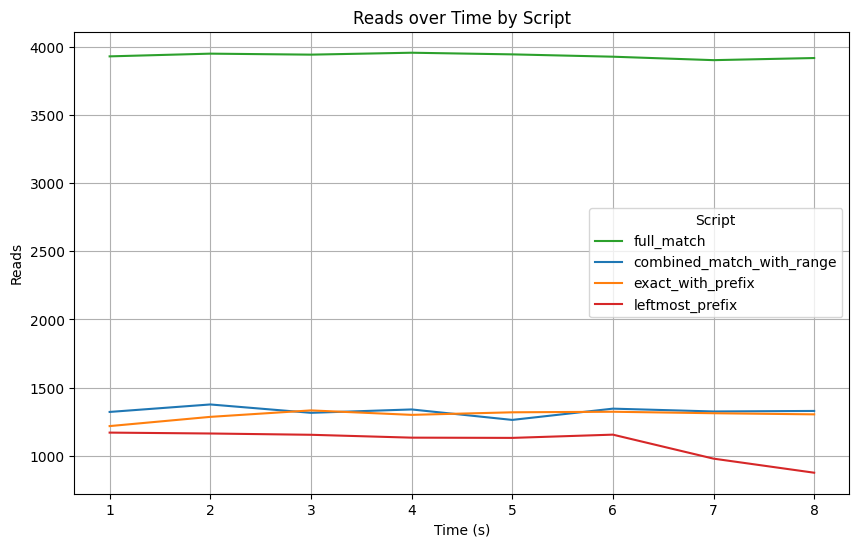
\includegraphics[width=\textwidth]{PNGs/Script/Index/Hash/hash-query-differences/Reads}
    \end{subfigure}
    \hfill
    \begin{subfigure}[t]{0.48\textwidth}
        \centering
        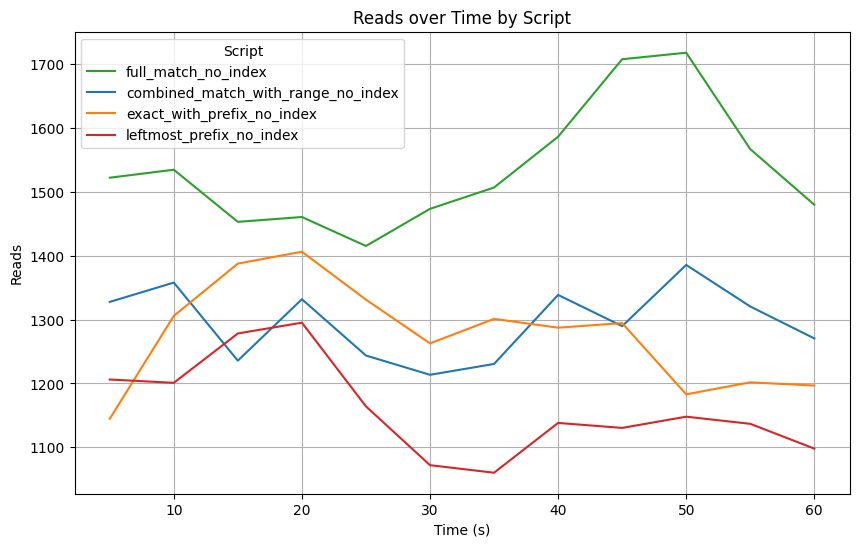
\includegraphics[width=\textwidth]{PNGs/Script/Index/Hash/hash-query-differences-no-index/Reads}
    \end{subfigure}
    \vspace{-8pt}
    \caption[Hash-Indexing: Unterschiedliche Abfragen mit Index und Ohne]{Grafik visualisiert Select-Queries mit (links) und ohne (rechts) Index}
    \label{fig:indexing-hash-query-reads}
\end{figure}

\section{Vergleich von B-Tree- und Hash-Index}\label{sec:indexing-comp-b-tree-hash-index}

In den vorherigen Kapiteln haben wir den B-Tree-Index und den Hash-Index jeweils getrennt voneinander betrachtet.
Dabei haben wir auch analysiert, bei welchen Select-Queries die Indizes Vorteile bringen und bei welchen nicht.
Damit fehlt uns noch der Vergleich zwischen dem B-Tree-Index und dem Hash-Index.

Um die Unterschiede zwischen beiden Indexstrukturen genauer zu analysieren, führen wir einen neuen Benchmark durch, der die Skripte aus Kapitel~\ref{sec:indexing-b-baum-index} und~\ref{sec:indexing-hash-index} wiederverwendet.
Da der Hash-Tree aber nur 4 unterschiedliche Select-Queries aufruft, wollen wir auch nur diese mit dem B-Tree-Index aufrufen.
Dazu fügen wir einfach den Parameter \texttt{selects} beim Aufruf des Orchestrator-Skripts hinzu und führen es anschließend aus.

\vspace{-4pt}
\begin{figure}[H]
    \centering
    \begin{subfigure}[t]{0.48\textwidth}
        \centering
        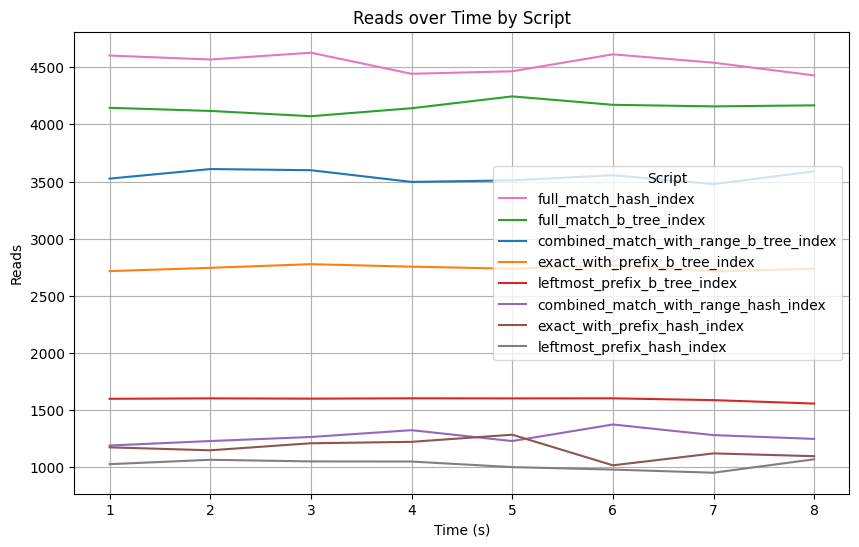
\includegraphics[width=\textwidth]{PNGs/Script/Index/B_Tree/hash-vs-b-tree-comparison/Reads}
        \caption{Anzahl der Lesezugriffe}
        \label{indexing-hash-vs-b-tree-comparison-reads}
    \end{subfigure}
    \hfill
    \begin{subfigure}[t]{0.48\textwidth}
        \centering
        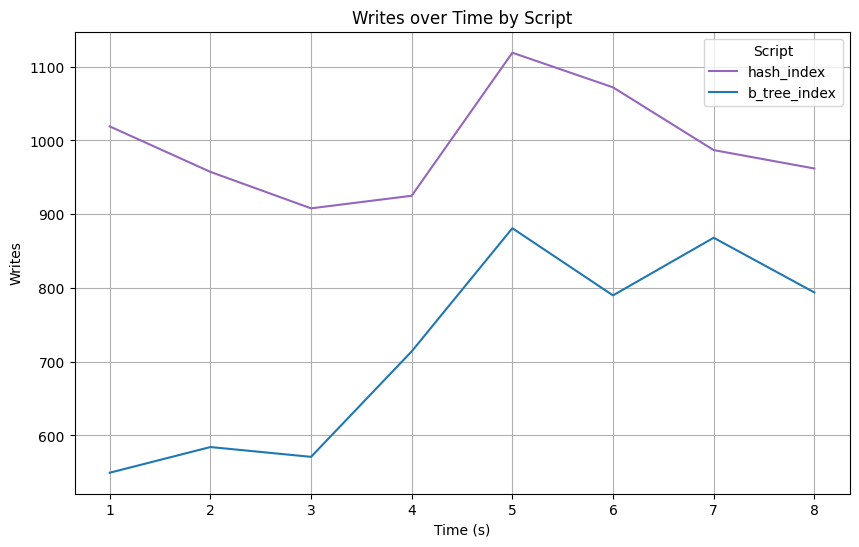
\includegraphics[width=\textwidth]{PNGs/Script/Index/B_Tree/hash-vs-b-tree-comparison/Writes}
        \caption{Anzahl der Schreibzugriffe}
        \label{indexing-hash-vs-b-tree-comparison-writes}
    \end{subfigure}
    \vspace{-2pt}
    \caption[Indexing: Vergleich von B-Tree- und Hash-Index]{Vergleich der Select-Query-Performance von B-Tree- und Hash-Index}
    \label{fig:indexing-hash-b-tree-comp}
\end{figure}
\vspace{-12pt}

In der Abbildung~\ref{indexing-hash-vs-b-tree-comparison-reads} sehen die Performance für die unterschiedlichen Select-Befehle.
Die höchste Transaktionsrate erzielt der Hash-Index, sofern der vollständige Schlüssel angegeben wird (\texttt{full\_match}).
Dicht darauf folgt der B-Tree-Index mit derselben Abfrage, allerdings mit etwa 10\% weniger Zugriffen.
Bei den übrigen Abfragen schneidet hingegen der B-Tree-Index deutlich besser ab, in einigen Fällen sogar bis zu dreimal schneller als der Hash-Index.
Den Grund dafür kennen wir schon aus den anderen Kapiteln.
Da der Hash-Index nur bei exaktem Schlüsselabgleich zum Einsatz kommt, wird er bei den anderen Abfragen nicht verwendet.
Mithilfe des \texttt{EXPLAIN}-Operators haben wir festgestellt, dass stattdessen der B-Tree-Index genutzt wird, was die starken Unterschiede erklärt.

Betrachtet man die Schreibperformance (Abbildung~\ref{indexing-hash-vs-b-tree-comparison-writes}), zeigt sich, dass der Hash-Index etwa 30--40\% schneller ist als der B-Tree-Index.
Wenn eine Anwendung also eine hohe Schreiblast hat, könnte der Hash-Index eine bessere Wahl sein, da er weniger Mehraufwand verursacht.
Zusammenfassend lässt sich festhalten, dass der Hash-Index einen leichten Vorteil hat, wenn beide Indexe greifen.
Andernfalls überwiegen die Stärken des B-Tree-Indexes.
